\documentclass[12pt,a4paper]{article}

\usepackage{graphicx}
\usepackage[left=1cm,right=1cm,top=1.5cm,bottom=1.5cm]{geometry}
\usepackage{listings}
\usepackage{lstlang-go}
\usepackage{jslistings}
\usepackage{solidity-highlighting}
% % Copyright 2017 Sergei Tikhomirov, MIT License
% https://github.com/s-tikhomirov/solidity-latex-highlighting/

\usepackage{listings, xcolor}

\definecolor{verylightgray}{rgb}{.97,.97,.97}

\lstdefinelanguage{Solidity}{
	keywords=[1]{anonymous, assembly, assert, balance, break, call, callcode, case, catch, class, constant, continue, constructor, contract, debugger, default, delegatecall, delete, do, else, emit, event, experimental, export, external, false, finally, for, function, gas, if, implements, import, in, indexed, instanceof, interface, internal, is, length, library, log0, log1, log2, log3, log4, memory, modifier, new, payable, pragma, private, protected, public, pure, push, require, return, returns, revert, selfdestruct, send, solidity, storage, struct, suicide, super, switch, then, this, throw, transfer, true, try, typeof, using, value, view, while, with, addmod, ecrecover, keccak256, mulmod, ripemd160, sha256, sha3}, % generic keywords including crypto operations
	keywordstyle=[1]\color{blue}\bfseries,
	keywords=[2]{address, bool, byte, bytes, bytes1, bytes2, bytes3, bytes4, bytes5, bytes6, bytes7, bytes8, bytes9, bytes10, bytes11, bytes12, bytes13, bytes14, bytes15, bytes16, bytes17, bytes18, bytes19, bytes20, bytes21, bytes22, bytes23, bytes24, bytes25, bytes26, bytes27, bytes28, bytes29, bytes30, bytes31, bytes32, enum, int, int8, int16, int24, int32, int40, int48, int56, int64, int72, int80, int88, int96, int104, int112, int120, int128, int136, int144, int152, int160, int168, int176, int184, int192, int200, int208, int216, int224, int232, int240, int248, int256, mapping, string, uint, uint8, uint16, uint24, uint32, uint40, uint48, uint56, uint64, uint72, uint80, uint88, uint96, uint104, uint112, uint120, uint128, uint136, uint144, uint152, uint160, uint168, uint176, uint184, uint192, uint200, uint208, uint216, uint224, uint232, uint240, uint248, uint256, var, void, ether, finney, szabo, wei, days, hours, minutes, seconds, weeks, years},	% types; money and time units
	keywordstyle=[2]\color{teal}\bfseries,
	keywords=[3]{block, blockhash, coinbase, difficulty, gaslimit, number, timestamp, msg, data, gas, sender, sig, value, now, tx, gasprice, origin},	% environment variables
	keywordstyle=[3]\color{violet}\bfseries,
	identifierstyle=\color{black},
	sensitive=false,
	comment=[l]{//},
	morecomment=[s]{/*}{*/},
	commentstyle=\color{gray}\ttfamily,
	stringstyle=\color{red}\ttfamily,
	morestring=[b]',
	morestring=[b]"
}

\lstset{
	language=Solidity,
	backgroundcolor=\color{verylightgray},
	extendedchars=true,
	basicstyle=\footnotesize\ttfamily,
	showstringspaces=false,
	showspaces=false,
	numbers=left,
	numberstyle=\footnotesize,
	numbersep=9pt,
	tabsize=2,
	breaklines=true,
	showtabs=false,
	captionpos=b
}
\usepackage{multirow}

\setlength{\parindent}{0em}

\begin{document}

\noindent
\begin{minipage}{120mm}
        {\huge {\bf School of Informatics}}\\
        {\Large {\bf Blockchains and Distributed Ledgers}}\\

        {\Large Assignment 3}\\
        {\normalsize Erodotos Demetriou (s2187344)}
\end{minipage}
\hfill
\begin{minipage}{40mm}              
        
\includegraphics[width=40mm]{crest.png}
\end{minipage}

\begin{center}
\rule{\linewidth}{0.5mm}
\end{center}

\section*{Part 1}

For Part A of this assignment, we are required to interact with a smart contract
deployed on the Ethereum Ropsten network. In more detail, we should call the
register method, giving input arguments a secret key and our student number.
Since Ethereum is a public blockchain, everything can be accessed on-chain.
Hence, the following script was used to retrieve the secret key from the smart
contract's storage. \\

\begin{lstlisting}[language=JavaScript]
const Web3 = require('web3');

var web3 = new Web3(new Web3.providers.HttpProvider('https://ropsten.infura.io/v3/0ab1814012ad4231965d67bf98a40b1a'));

var contract_address = '0xde3a17573B0128da962698917B17079f2aAbebea';

web3.eth.getStorageAt(contract_address, 1).then(result => {
    console.log(web3.utils.hexToString(result));
});
\end{lstlisting} 

\vspace{5mm}

The found key is: "actually...;)". We imported the smart contract source code
and address into \emph{Remix} and finally called the register function with
"actually...;)" and "s2187344" as inputs. \\

Transaction Hash : 0xc6ebbfea38258b115d07d5826667dfdd2445a5cbe277f0c3e18fa5a294ef3d32

\section*{Part 2 A}

\subsection*{Smart Contract High-Level Description}

Part 2 A of this assignment regards implementing and deploying a custom token.
Its requirements include allowing users to exchange ETH for tokens, sell their
tokens back for ETH, and transfer tokens between accounts. Also, the users can
view their balance by calling the smart contract. Besides that, the token owner
can change the token's price if there is enough balance in the smart contract. \\

To achieve that, we introduced the concept of liquidity providers. Liquidity
providers are individuals willing to deposit their ETH to the smart contract and
receive tokens as rewards whenever a new buyer purchases the token in the
future. Next, we provide a real-world example of using this mechanism to
understand its functionality better. \\

\begin{figure}[htpb]
    \begin{center}
        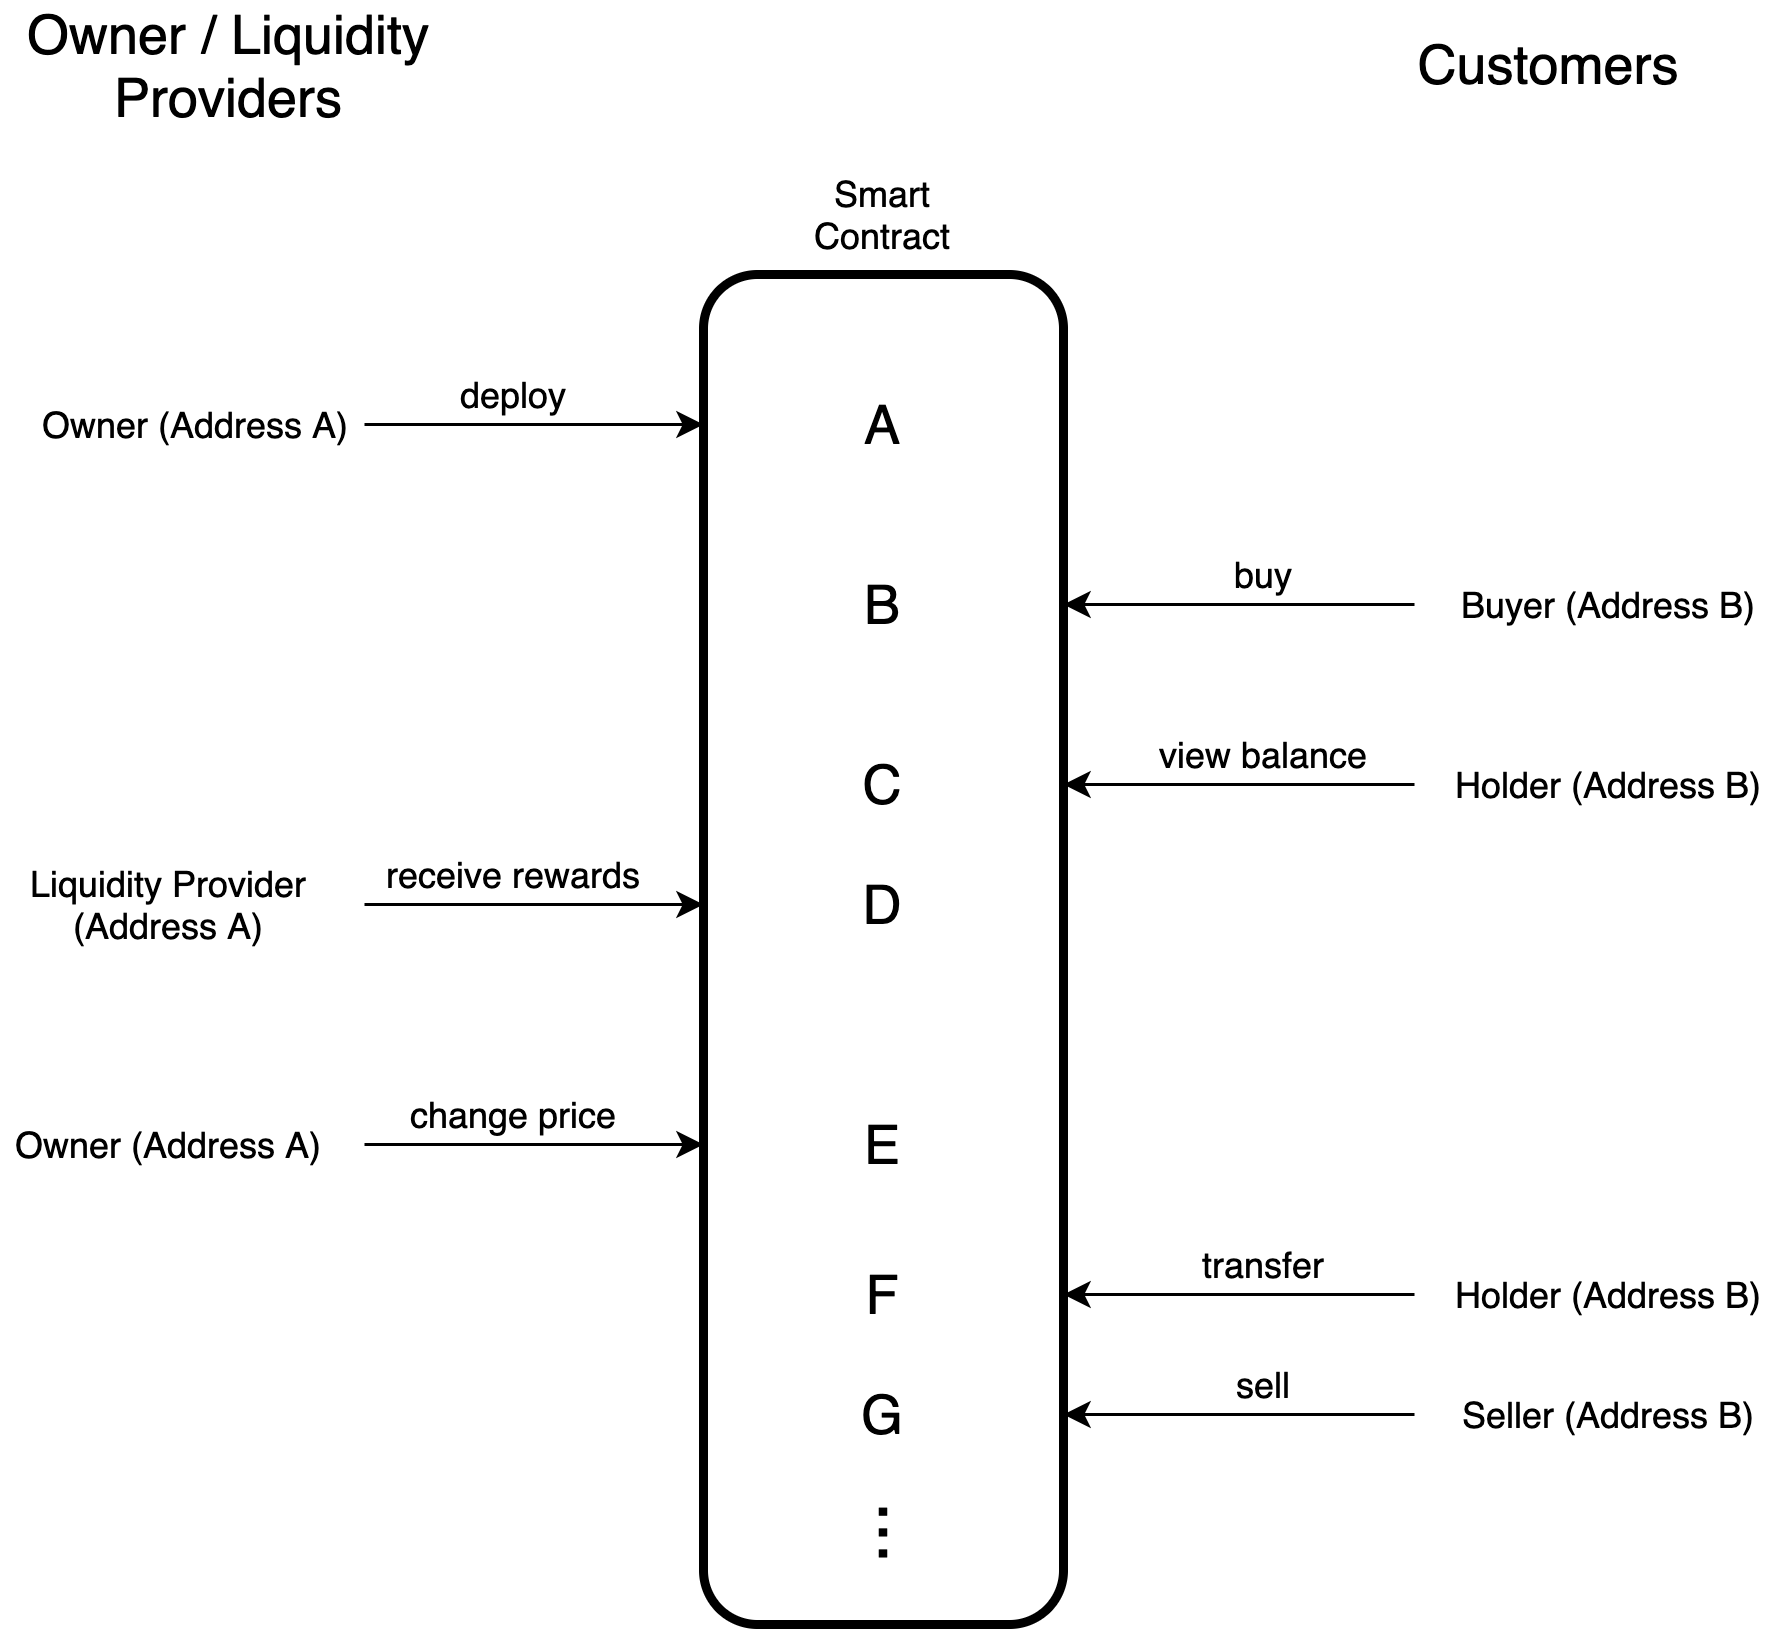
\includegraphics[height=8cm]{execution_flow.png}
        \caption{Smart Contract Execution Workflow Example}
        \label{fig:smart-contract-example}
    \end{center}
\end{figure} 

Figure \ref{fig:smart-contract-example} illustrates the smart contract's life cycle. In
step A, the owner (address A) deploys the smart contract providing 100 Wei. This
automatically registers him as the first liquidity provider. Next, in step B, we
can observe a buyer (address B) conducting a buy request to the smart contract.
For instance, he wants to buy 30 tokens priced at 10 Wei each. Hence, he has to
send 300 Wei to the smart contract and provide the number of tokens as an input
parameter. We check for the validity of the input data, and if everything is
accurate, we proceed. 10\% of the purchased tokens is contributed into a rewards
pool while the customer receives 90\%. We have to mention that for simplicity
objectives in calculating the percentage, we allow purchases of multiples of 10.
Later, in step C the buyer can view its balance by calling the getBalance()
method of the smart contract. At this point (D), a liquidity provider can
receive rewards from the rewards pool. He will get a portion of tokens according
to the fraction of liquidity he provided to the total liquidity.
Each provider can increase the rewards he receives by offering more liquidity.\\

Nonetheless, we have to note that because solidity does not support floats, we
restrict the amount a liquidity provider can offer to multiples of 100 Wei.
Further, if there is only one token in the rewards pool and two liquidity
providers own 50\% of it each, the smart contract will not allow them to receive
rewards because of an impossible division of 1/2. They can receive their rewards
later when the pool balance allows a fair distribution. \\

Now, suppose we want to change the price of our token. The owner can allow this
action in step E. The only constrain of this transaction is that the contract's
balance should be greater or equal to the product of circulating tokens and the
new price. \\

Moreover, a token holder can transfer its tokens to another address. This is
depicted in step F, where the user calls the smart contract providing the
receiver's address and the amount of tokens. \\

Finally, any token holder may sell his tokens to the smart contract for ETH
considering the current token price in Wei. The sellToken function does not
directly transfer ETH to the user. Instead, a custom library deployed on the
Ropsten network is used. One of the main challenges of this assignment was to
link an already deployed library into our smart contract. This was impossible to
achieve through \emph{Remix} online editor. Thus we used \emph{Truffle} smart contract
development framework to achieve the desired outcome. Practically, we compiled
the customLib.sol locally to generate a reference ABI and afterward import the
library into our Token.sol contract. Since we needed to use an already deployed
instance of the library, we specified its address in the migrations javascript
file and used the link method to reference it. There follows the deployment and
link code for the operation as mentioned earlier and a detailed overview of smart
contract's variables, functions and events. \\

\pagebreak

\begin{lstlisting}[language=JavaScript]
const Token = artifacts.require("Token");
const CustomLibrary = artifacts.require("customLib");

module.exports = function(deployer, accounts) {
    CustomLibrary.address = "0xc0b843678E1E73c090De725Ee1Af6a9F728E2C47"
    deployer.link(CustomLibrary, Token);
    deployer.deploy(Token, { value: "100" })
};
\end{lstlisting}

\textbf{\underline{Variables}} \\
\textbf{\emph{address owner:}} This variable is set on deployment, and stores the smart
contract's owner address.\\
\textbf{\emph{uint256 contractBalance:}} This variable stores the number of Wei deposited
into the smart contract.\\
\textbf{\emph{uint256 circulatingTokens:}}  This variable stores the number of
circulating tokens.\\
\textbf{\emph{mapping balances:}} This is a mapping variable maintaining a one to one
correspondance between a user address and the number of tokens it holds. \\
\textbf{\emph{mapping liquidityProviders:}} This is a mapping variable maintaining a one
to one correspondance between a liquidity provider user address and the amount
of liquidity it provided in \emph{wei}. \\
\textbf{\emph{uint256 numberOfProviders:}} This variable holds the number of total
liquidity providers.\\
\textbf{\emph{uint256 totalLiquidity:}} This variable holds the amount of total liquidity
provided during the complete life cycle of the smart contract.\\
\textbf{\emph{uint256 rewardsPool:}} This variable stores the amount of tokens that will
be available to liquidity providers as rewards for their services.\\
\textbf{\emph{uint256 tokenPrice:}} This variable stores the current token price in Wei.\\

\textbf{\underline{Events}} \\
\textbf{\emph{event Purchase:}} Whenever a token purchase is fulfilled, an event stating
the buyer's address and the purchased amount, is emitted.\\
\textbf{\emph{event Sell:}} Whenever a token holder sells its tokens back to the smart
contract, a sell event is emitted. This event states the seller address and the
amount of tokens sold.\\
\textbf{\emph{event Transfer:}} Whenever a token holder transfers its tokens to an other
address a transfer event is emitted. This event states the sender and receiver
adddresses, as well as the transfered amount of tokens.\\
\textbf{\emph{event Price:}} This event is emitted whenever the smart contract owner
changes the token price.\\

\textbf{\underline{Functions}} \\
\textbf{\emph{constructor():}} This is the smart contract constractor. It is
called whenever the code is deployed for the first time, and sets the contract
owner, as the initiator of the transaction. The smart contract constructor
requirement is that the owner provides 100 Wei as initial liquidity. In
other words, he becomes the first liquidity provider.\\
\textbf{\emph{buyToken():}} Whenever a buyer wants to exchange his ETH for our token has
to call this function. In more detail, he needs to provide as input the number
of tokens that he desires to purchase and send the proportional amount of ETH,
considering the token price which is in Wei.\\
\textbf{\emph{transfer():}} This function can be called by a token holder that desires to
transfer a specific amount of tokens to an other address.\\
\textbf{\emph{sellToken():}} This function enables a token holder to exchange his tokens
with ETH. He can provide the number of tokens he wants to exchange and
subsequentyl he will receive the according value of ETH considering the current
token price.\\
\textbf{\emph{changePrice():}} This function can be called only by the smart contract
owner, to change the token price. Its execution will only succed if there is
enough liquidity to pay token holders if they decide to sell their token
simultaneously.\\
\textbf{\emph{getBalance():}} This function returns the balance of tokens that are in the
posetion of the fucntion's caller.\\
\textbf{\emph{provideLiquidity():}} This is an internal function that can be triggered
through the fallback function. It receives an address and the amount of provided
liquidity. Subsequently, it registers this user as a liquidity provider. \\
\textbf{\emph{getReward():}} This is an internal function that can be trigered through
the fallback function and only if the caller is a registered liquidity provider.
Its execution results into receiving a proportion of the reward tokens from the
reward pool.\\
\textbf{\emph{fallback():}} This function can be used with different arguments and can
serve different purposes. If it is called providing some ETH, registers the user as a
liquidity provider; else, it can be used by liquidity provider to receive its
rewards.

\subsection*{Gas Costs Evaluation}
This section measures and evaluates the gas cost we expect to have when deploying and
interacting with the smart contract. \\

Gas costs appear in the following table. The smart contract owner has to pay
1,389,915 gas units to deploy the code. This is a high amount of gas, making the
smart contract expensive to deploy initially. Using the already deployed library
save us only 39,400 gas which is not much. \\

\begin{table}[htpb]
    \begin{center}
        \begin{tabular}{cc}
        \multicolumn{2}{c}{\textbf{Gas Costs}}                                                                \\
        \multicolumn{1}{l}{}                                                & \multicolumn{1}{l}{}            \\ \hline
        \multicolumn{2}{|c|}{\textit{\textbf{Contract Owner Fees}}}                                           \\ \hline
        \multicolumn{1}{|c|}{Contract Deployment (lib)}                     & \multicolumn{1}{c|}{1,389,915}  \\ \hline
        \multicolumn{1}{|c|}{Contract Deployment (no-lib) }                 & \multicolumn{1}{c|}{1,429,315}  \\ \hline
        \multicolumn{1}{l}{}                                                & \multicolumn{1}{l}{}            \\ \hline
        \multicolumn{2}{|c|}{\textit{\textbf{Customer Fees}}}                                                 \\ \hline
        \multicolumn{1}{|c|}{buyToken()}                                   & \multicolumn{1}{c|}{65,102}   \\ \hline
        \multicolumn{1}{|c|}{sellToken()}                                  & \multicolumn{1}{c|}{62,875}   \\ \hline
        \multicolumn{1}{|c|}{transfer()}                                   & \multicolumn{1}{c|}{52,328}   \\ \hline
        \multicolumn{1}{|c|}{changePrice()}                                & \multicolumn{1}{c|}{34,639}   \\ \hline
        \multicolumn{1}{|c|}{getBalance()}                                 & \multicolumn{1}{c|}{None}   \\ \hline
        \multicolumn{1}{l}{}                                               & \multicolumn{1}{l}{}             \\ \hline
        \multicolumn{2}{|c|}{\textit{\textbf{Liquidity Provider Fees}}}                                       \\ \hline   
        \multicolumn{1}{|c|}{provideLiquidity()}                           & \multicolumn{1}{c|}{42,083}   \\ \hline
        \multicolumn{1}{|c|}{getReward()}                                  & \multicolumn{1}{c|}{35,110}   \\ \hline
        \end{tabular}
    \end{center}
\end{table}

Regarding the smart contract customers interactions, the fees are much lower.
Namely, when buying some tokens, the gas required is 65,102, while the
invocation of sellToken function costs 62,875. We can observe that buying and
selling tokens from and to the contract yields approximately the same overhead.
Next, if a token holder transfers its tokens to another address, he can use only
52,328 gas units, which is relatively cheap. Retrieving the available balance of
tokens for a specific address occurs at no expense. \\

Besides customer invocations, we have liquidity providers interacting with the
smart contract. Providing liquidity costs 42,083 gas units. When designing the
provide liquidity functionality, our goal was to keep it as cheap as possible to
motive liquidity providers to back the token sale. We can argue that this has
partially been achieved since depositing funds is cheaper than buying or selling
tokens. Furthermore, when a liquidity provider requests its rewards, the costs
are even cheaper at 35,110 gas units. Nonetheless, a liquidity provider will
amortize its investment with more profits since 10\% of each token purchase goes
to him.

\pagebreak

\subsection*{Potential Hazards and Vulnerablities}

Developing a Smart Contract can always be challenging. This is because, on a
public-permissionless blockchains, everything is observable by everyone. This
fact makes it difficult when it comes to securing users’ data. Besides that, a
developer has to be alert to write code that is attack-resistant. Smart
contracts expose a broad spectrum of vulnerabilities, enabling an adversarial
entity to exploit them for his interest.\\

When developing our custom token, we took into consideration possible
attacks. The following list presents vulnerabilities and mechanisms to moderate
them. \\

\textbf{\emph{DoS(Denial of Service) - Griefing: }}An attacker attempts to make
a Smart Contract get stuck when executed. In the case of our implementation, we
don't face such problems. The nature of the code does not allow the contract to
get stuck. All functions are atomic, which means that they will complete or
fail. The only scenario in which we might face grief in our smart contract is
when there is insufficient liquidity to change that token price. In other words,
if there are not enough liquidity providers, the contract owner won't be able to
increase the token price frequently. Similarly, if don't have buyers, liquidity
providers won't receive rewards and thus lose their initial investment. \\

\textbf{\emph{Mitigation: }}To mitigate this issue, we require that the
contract owner provide initial liquidity to the smart contract by becoming the
first liquidity provider. \\

\textbf{\emph{Re-Entrancy: }}An attacker might try to take advantage of the
smart contract sellToken function by executing a re-entrancy attack. In more
detail, when he invokes a sellToken transaction, he can drive his transaction
to a malicious fallback function on another Smart Contract that can recursively
call again and again the sellToken function, trying to get more ETH.\\

\textbf{\emph{Mitigation: }}In order to avoid such unpleasant attacks, we
execute the code of the smart contract in a particular way. When there is a
withdrawal invocation, we check some constraints to ensure that the transaction
sender is allowed to withdraw ETH. After that, we will pass any updates to the
state of the smart contract and eventually make the call that sends the
requested ETH to the recipient. It is essential to make the ETH transfer after
changing the smart contract state. If a reentrancy attack occurs on the next
transaction, it will be stopped because function constraints will evaluate the
transaction according to the updated state.\\

\textbf{\emph{Front-Running: }} This attack happens on the Miner level. An
attacker might clone your transaction and put a much higher gas limit on it.
This results in including his transaction in the next block instead of yours.
This might be inconvenient when a buyer tries to buy some tokens priced at 10
Wei, and the smart contract owner front-runs him to increase the price. Further,
we have to note that our token has no limited supply, and thus, there is no
meaning in front-running its purchase. Everyone can buy any amount of tokens. \\

\textbf{\emph{Mitigation: }}There is no straightforward solution to
front-running since the problem lies at the transaction mining level. For our
custom token, front-running will not have a significant effect. \\

\textbf{\emph{Overflow/Underflow: }} Our custom token does not face this problem
since it is coded using version 0.8.0 of Solidity, which automatically resolves
any issues of over/under flow and aborts the execution of the smart contract.\\

\textbf{\emph{Randomness Source Exposure: }} Our custom token does not involve
using any random value. \\

\textbf{\emph{Delegation: }}In our smart contract, we used a custom library to
send funds to an address when a sale occurs. We assume that this library is safe
as the assignment authors have provided it. \\

\textbf{\emph{\underline{Other good practices:}}}

\begin{itemize}
    \item Use \emph{call()} instead of \emph{transfer()} or \emph{send()}. Using
    \emph{call()}  might be insecure, but \emph{transfer()} and \emph{send()}
    can forward only 2300 gas. In the future gas costs might change, and 2300
    gas might not be enough. As a result, using \emph{call()} properly is the
    right approach. We use a custom library that uses call() to send ETH; thus,
    we check its output correctness, as shown in the example below.\\
    \begin{lstlisting}[language=Solidity]
        (bool success = customLib.customSend(amount * tokenPrice, msg.sender);
        require(success, "Transfer failed!");
    \end{lstlisting}
    \item A liquidity provider might want to receive its rewards. For this part
    of the implementation, we decided it is safer for the smart contract to have
    an external user initiate the reward distribution, instead of pushing the
    tokens into his address. In other words we have them pulling their rewards.
    \item As for our fallback function, we keep it simple, allowing only two
    operations. It can only be used to provide liquidity or receive rewards. Any
    other operation on the smart contract's fallback functions will result in a
    deadlock.
    \item Moreover, it is an excellent practice to emit events when a critical
    transaction is complete. Hence, we emit events whenever a token sale,
    purchase, or transfer occurs.
\end{itemize}

\subsection*{Smart Contract Deployment and Execution History}

\textbf{Owner Address:} 0x1959f7433D617977e144cC3Bb722D794384D562B

\begin{itemize}
    \item \textbf{Smart Contract deployment}\\
    TX Hash: 0x5ba0d9a48485c1400f72bf2d0482b869f44935ceb38cbb8a720a5d66c391ece0 \\
    Contract Address: 0x8252e289f6ef096CCb0647322102ac5459D1Df49
    \item \textbf{Buy Tokens}\\
    TX Hash: 0xeaf2f20e09dc42dbf743d6edd7618e831f3ce195967ccb4624b4b6dfa395ab88
    \item \textbf{Get Rewards}\\
    TX Hash: 0x7aef6df0c8b4a3d8f7685c3e7cc2f33117addeea284d0fd940abbab9e17c60b7
    \item \textbf{Change Price}\\
    TX Hash: 0xae26b213a00cd543b3a57e97d9f0626b18812df69fb10cc843432302442f122a
    \item \textbf{Transfer Tokens}\\
    TX Hash: 0xfa2a9b619d58b934957503f8afdd08ceafcd71e228d7d27fc357c8ad4b3c1976
    \item \textbf{Sell Token}\\
    TX Hash: 0x53be3484f8fe51bd58bc5f4aec9f0ae45711b7b8924c23f70f512ba21f0c5aa1
    \item \textbf{Provide Liquidity}\\
    TX Hash: 0x43f228412eb74dc55e40c95f5f020e4efe3bdc4b6eef91dda21a2041f08dd002
\end{itemize}

\pagebreak

\subsection*{Implementation Code}
\begin{lstlisting}
pragma solidity >=0.8.00 <0.9.0;

import "./customLib.sol";

contract Token {
    address private owner;
    uint256 private contractBalance = 0;
    uint256 private circulatingTokens = 0;
    mapping(address => uint256) private balances;
    mapping(address => uint256) private liquidityProviders;
    uint256 private numberOfProviders = 0;
    uint256 private totalLiquidity = 0;
    uint256 private rewardsPool = 0;
    uint256 public tokenPrice = 10;
    event Purchase(address indexed buyer, uint256 amount);
    event Sell(address indexed seller, uint256 amount);
    event Price(uint256 price);
    event Transfer(
        address indexed sender,
        address indexed receiver,
        uint256 amount
    );
    constructor() payable {
        require(
            msg.value == 100,
            "As the contract owner you are required to provide 100 wei liquidity"
        );
        owner = msg.sender;
        provideLiquidity(owner, msg.value);
    }

    function buyToken(uint256 amount) public payable returns (bool) {
        require(
            msg.value == amount * tokenPrice,
            "Your funds are not sufficient"
        );
        require(
            amount % 10 == 0,
            "The purchased quantity should be multiple of 10!"
        );
        circulatingTokens += amount;
        contractBalance += amount * tokenPrice;
        balances[msg.sender] += (amount * 90) / 100;
        rewardsPool += (amount * 10) / 100;
        emit Purchase(msg.sender, amount);
        return true;
    }

    function transfer(address recipient, uint256 amount) public returns (bool) {
        require(balances[msg.sender] >= amount, "Not enough balance");
        balances[msg.sender] -= amount;
        balances[recipient] += amount;
        emit Transfer(msg.sender, recipient, amount);
        return true;
    }

    function sellToken(uint256 amount) public returns (bool) {
        require(amount >= 1, "Provide positive amount of tokens!");
        require(amount <= balances[msg.sender], "Not enough balance!s");
        require(amount > 0, "Not enough balance!");
        circulatingTokens -= amount;
        balances[msg.sender] -= amount;
        contractBalance -= amount * tokenPrice;
        bool success = customLib.customSend(amount * tokenPrice, msg.sender);
        require(success, "Transfer failed!");
        emit Sell(msg.sender, amount);
        return true;
    }

    function changePrice(uint256 price) public returns (bool) {
        require(
            msg.sender == owner,
            "This function is restricted to the contract's owner"
        );
        require(
            contractBalance >= circulatingTokens * price,
            "Not enough liquidity"
        );
        tokenPrice = price;
        emit Price(price);
        return true;
    }

    function getBalance() public view returns (uint256) {
        return balances[msg.sender];
    }

    function provideLiquidity(address provider, uint256 amount) internal {
        liquidityProviders[provider] += amount;
        totalLiquidity += amount;
        contractBalance += amount;
        numberOfProviders += 1;
    }

    function getReward() internal {
        require(
            liquidityProviders[msg.sender] >= 100,
            "You are not a liquidity provider"
        );
        require(
            rewardsPool % numberOfProviders == 0,
            "You can not receive rewards now (unfair division)"
        );
        uint256 allowance = (liquidityProviders[msg.sender] / totalLiquidity) *
            100;
        balances[msg.sender] += (rewardsPool * allowance) / 100;
        rewardsPool -= (rewardsPool * allowance) / 100;
    }

    fallback() external payable {
        if (msg.value > 0) {
            provideLiquidity(msg.sender, msg.value);
        } else {
            getReward();
        }
    }
}
\end{lstlisting}

\section*{Part 2 B}

KYC, also known as  "know your customer", is common practice among financial
institutions when a new client enters their business. They use KYC to verify the
client's identity and evaluate the risks of maintaining a business relationship.
A straightforward KYC methodology might include submitting an identification
document such as a birth certificate, proof of address of a legitimate utility
bill, and a recent face photograph of the client. Within the context of Part 2 B
of this assignment, we need to describe such a mechanism for our custom token
sale. Further, we will argue if this is feasible to implement on the blockchain. \\

It is more than evident that having many customers yields a requirement for
storing thousands of documents. The Ethereum blockchain is not the best option
for storing documents. Foremost, we can not directly store multimedia such as
pdf files and images on-chain. We should convert them into an intermediate text
form such as base64 encoding. This is going to add computational overhead.
Moreover, storing 1KB of data requires approximately 640K gas which is not
cheap. Besides that, Ethereum is a public permissionless blockchain, thus
storing KYC documents on-chain can violate the customers' privacy. Hence in our
KYC  proposal, we attempt to instrument a hybrid solution using both blockchain
and a centralized server to process new customer requests. The main idea of our
implementation is that a new customer submits its documents on the server for
approval while publishing its KYC identification fingerprint on-chain.
Afterward, the smart contract owner reviews the submitted documents off-chain,
and if they are valid, he can approve them and enable the client to purchase
tokens on-chain. There follows a more thorough explanation. \\


When designing the KYC mechanism, the foremost priority was user data privacy,
and gas efficiency and fairness. For this reason, we adopt a public-key
cryptography scheme to encrypt identification documents and sign them. To
achieve that, we introduce a central trusted authority that keeps the public
keys of both contract owner and client. When a new customer wants to initiate a
KYC procedure, follows the steps below, as depicted in Figure \ref{fig:kyc-process}

\begin{enumerate}
    \item Clients and the contract owner publish their public keys to the trusted authority.
    \item Clients and the contract owner retrieve public keys of the entity they
    desire from the trusted authority.
    \item The server publishes a Nonce that encrypts using the client's public
    key and sends it to the client, as a challenge, to include in its subsequent
    KYC request. The client decrypts the Nonce using its private key.
    \item The user prepares a PDF file, including its identification documents.
    We call this, Data. Next, the user concatenates Data and the received Nonce
    and encrypts them using the server's public key, producing a Ciphertext.
    Then he signs the Ciphertext by hashing it and encrypting it using his
    private key.
    \item In step 5, the user forwards the signed Ciphered text to the server
    while publishing its signature/fingerprint on-chain.
    \item The server receives the signed Ciphertext and proceeds to validate it.
    Mainly, we check for Nonce validity and Data (documents) validity and
    signature.
    \item We retrieve the on-chain recorded signature and perform a peculiar
    3-way check, comparing the submitted to server signature with the
    recalculated Ciphertext Hash and the signature submitted on-chain.
    \item If everything is valid, the contract owner can proceed and approve the
    client's requests to purchase tokens from the smart contract. 
\end{enumerate}

We decided to introduce the concept of a nonce to avoid replay attacks when
submitting the identification documents to the server. Further, we have both
client and owner interacting with the smart contract, splitting the gas costs of
completing the KYC process. This approach provides gas fairness and transparency
to the client, ensuring that its digital fingerprint/signature is correct. This
is important since that digital fingerprint associates the client with an
encrypted form of its KYC documents.\\

Indubitably, we have to extend our smart contract's public  API to support the
mechanism above. This hybrid KYC tool requires very few changes to the smart
contract, narrowing the gas costs required to implement it. In more detail, we
need the following function and variables.\\

\begin{lstlisting}[language=Solidity]
    mapping(address => KYC) public kyc;
    struct KYC {
        bytes64 finger_print ;
        bool approved;
    }
    function setFingerPrint(bytes64 finger_print) public returns (bool);
    function getFingerPrint(address client_address) public returns (bytes64);
    function approveClient(address client_address) public returns (bool);
\end{lstlisting}

Finally, we need to add a requirement statement into the buyToken function to
check if the client's address is approved.  \\

\begin{lstlisting}[language=Solidity]
    require(kyc[msg.sender].approved == True, "Your are not allowed to buy tokens");
\end{lstlisting}

\begin{figure}[htpb]
    \begin{center}
        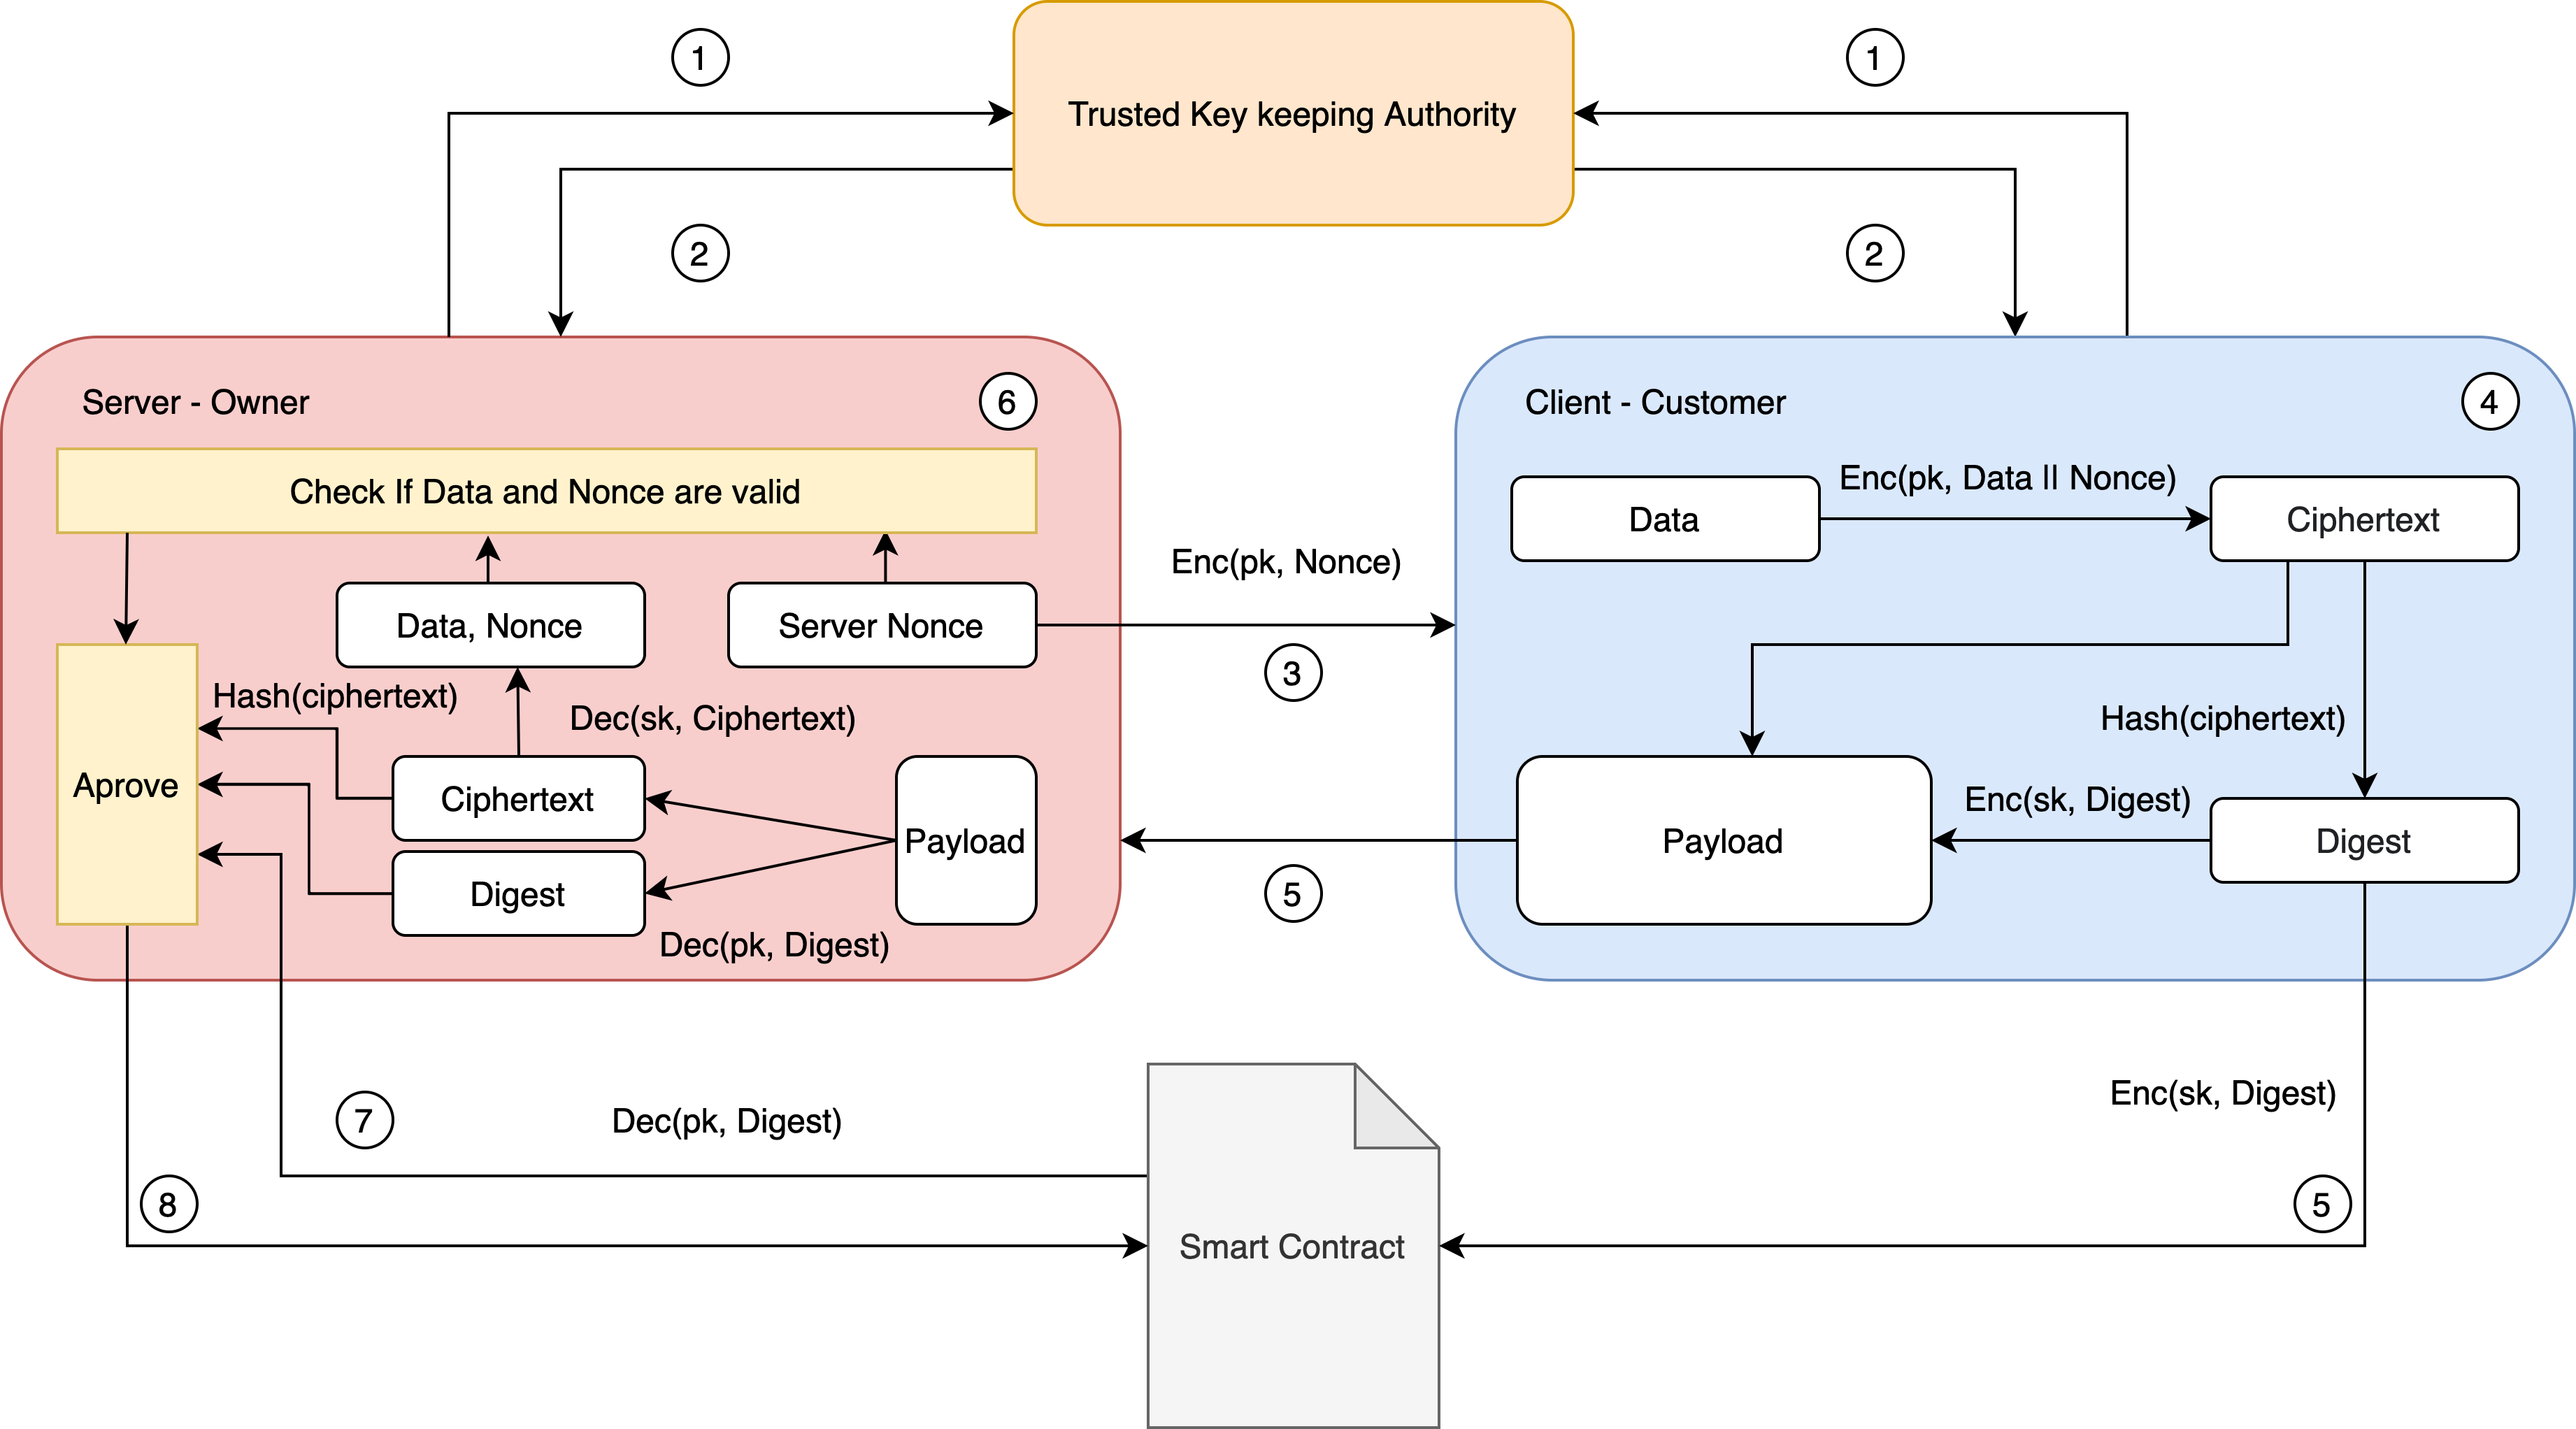
\includegraphics[width=18cm]{kyc.png}
        \caption{KYC process}
        \label{fig:kyc-process}
    \end{center}
\end{figure} 
\end{document}